\documentclass[conference]{IEEEtran}
\usepackage{amsmath,amssymb,amsfonts}
\usepackage{xcolor}
\usepackage{tikz,pgfplots}
\usetikzlibrary{positioning}
\usetikzlibrary{arrows}
\usetikzlibrary{patterns}
\usetikzlibrary{shapes.geometric}

\begin{document}

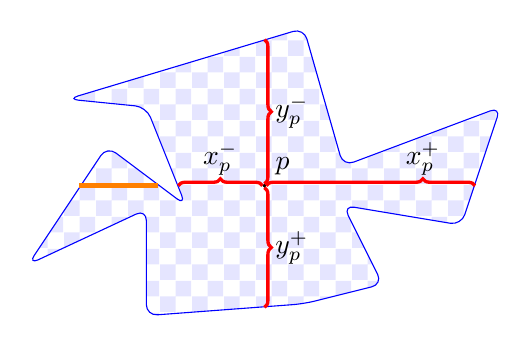
\begin{tikzpicture}
\draw[blue, pattern=checkerboard, pattern color=blue!10, rounded corners] (-3, -1) --
 (-2, 0.5) -- (-1, -0.25) -- (-1.5, 1) -- (-2.5, 1.1) -- (0.5, 2) -- (1, 0.25) -- (3, 1) -- (2.5, -0.5) -- (1, -0.25) -- (1.5, -1.25) -- (0.5, -1.5) -- (-1.5, -1.65) -- (-1.5, -0.3) -- cycle;
 
\node[inner sep=0pt, circle, draw, fill=black] at (0, 0) (p) {};
\node[above right=0 of p] {$p$};

\draw[-, red, very thick, decorate, decoration={brace, mirror, aspect=0.5}] (p.west) -- +(-1.07, 0) node[pos=0.5, above=0pt, black]{$x^-_p$};
\draw[-, red, very thick, decorate, decoration={brace, aspect=0.75}] (p.east) -- +(2.65, 0) node[pos=0.75, above=0pt, black]{$x^+_p$};
\draw[-, red, very thick, decorate, decoration={brace, mirror, aspect=0.5}] (p.north) -- +(0, 1.83) node[pos=0.5, right=0pt, black]{$y^-_p$};
\draw[-, red, very thick, decorate, decoration={brace, aspect=0.5}] (p.south) -- +(0, -1.52) node[pos=0.5, right=0pt, black]{$y^+_p$};

\draw[-, orange, ultra thick] (-1.35, 0) -- +(-1, 0);
\end{tikzpicture}

\end{document}